% OLD VERSION
% \jh{A little too technical?}
% The key difference between FEP and thermodynamic integration is that we can analytically compute the derivative of the changing potential with respect to the perturbation parameter (lambda) and integrate numerically. 
% As such, we don't need to keep track of energy differences directly but simply sample the value of the collective variable regularly while the force constant is gradually reduced to 0.
% Implementation details can be found in the provided configuration files and in section \ref{step:restraint-perturbation} of the protocol.

% During the RFEP, the force constant is made dependent on a perturbation parameter $\lambda$ between 0 and 1.
% To improve numerical behavior around $\lambda = 0$, we use a non-linear dependence:
% \begin{equation}\label{eq:kl}
%     k_\lambda = k_0 + \lambda^\alpha (k_1-k_0)
% \end{equation}
% where the exponent $\alpha$ is defined by the Colvars parameter \texttt{targetForceExponent}, and set to 6 in the present example.

% With these data and some information about the way the TI calculation was carried out, not only can we estimate the free energy cost of imposing the restraint, but also assign an error to that estimate - a task which is not always trivial.
% Combining Equations \ref{eq:harmonic_wall} and \ref{eq:kl} and taking the partial derivative with respect to $\lambda$ yields:
% \grace{update notation}\ezry{I'm pretty sure this is the notation we agreed on. Is this an old note?}
% \begin{equation}\label{eq:dUwalldlambda}
%     \frac{\partial}{\partial \lambda} U_\mathrm{FB}(r) =\begin{cases}
%         \frac{1}{2}a\lambda^{a-1}(k_1 - k_0)(r-r_\mathrm{R})^2&, r>r_\mathrm{R}\\
%         0 &, \text{otherwise}
%     \end{cases} 
% \end{equation}
% Where $k_0 = 0$ (\texttt{forceConstant}), $k_1$ is the final force constant (\texttt{targetForceConstant}), $r$ is the DBC, and $r_\mathrm{R}$ is the upper wall of the DBC restraint. 
% Equation \ref{eq:dUwalldlambda} is applied to the colvars trajectory data in the Jupyter notebook section associated with step C. 
% Finally, we estimate the free energy difference between the endpoints $\lambda=0$ and $\lambda=1$ using Equation \ref{eq:TI}. The error in the final estimate is obtained from the standard deviation of each mean. A tighter estimate of the error can be obtained by running replicas for the TI calculation.

% \begin{equation} \label{eq:TI}
%     \Delta G = \sum_{\lambda=0}^1 \left\langle
%     \frac{\partial U(\lambda)}{\partial \lambda}\right\rangle
% \end{equation}

% \begin{figure}[ht]
% 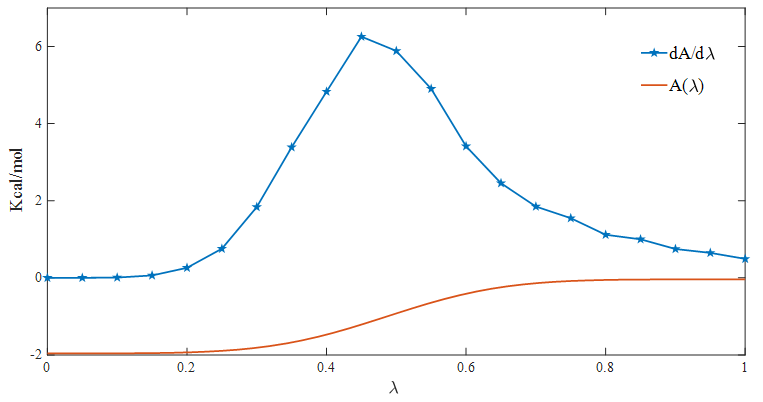
\includegraphics[width=0.99\linewidth]{RFEP}
% \caption{Restraint free energy ($A(\lambda)$, red line) and its derivative with respect to the coupling parameter ($dA/d\lambda$, blue line), as a function of $\lambda$.}\label{fig:RFEP2}
% \end{figure}
